\documentclass{article}

\usepackage{arxiv}

\usepackage[utf8]{inputenc} % allow utf-8 input
\usepackage[T1]{fontenc}    % use 8-bit T1 fonts
\usepackage{hyperref}       % hyperlinks
\usepackage{url}            % simple URL typesetting
\usepackage{booktabs}       % professional-quality tables
\usepackage{amsfonts}       % blackboard math symbols
\usepackage{nicefrac}       % compact symbols for 1/2, etc.
\usepackage{microtype}      % microtypography
\usepackage{lipsum}
\usepackage{graphicx}
\usepackage{float}

\usepackage{listings}
\usepackage{xcolor}

\definecolor{codegreen}{rgb}{0,0.6,0}
\definecolor{codegray}{rgb}{0.5,0.5,0.5}
\definecolor{codepurple}{rgb}{0.58,0,0.82}
\definecolor{backcolour}{rgb}{0.95,0.95,0.92}

\lstdefinestyle{mystyle}{
    backgroundcolor=\color{backcolour},   
    commentstyle=\color{codegreen},
    keywordstyle=\color{magenta},
    numberstyle=\tiny\color{codegray},
    stringstyle=\color{codepurple},
    basicstyle=\ttfamily\footnotesize,
    breakatwhitespace=false,         
    breaklines=true,                 
    captionpos=b,                    
    keepspaces=true,                 
    numbers=left,                    
    numbersep=5pt,                  
    showspaces=false,                
    showstringspaces=false,
    showtabs=false,                  
    tabsize=2
}

\lstset{style=mystyle}

\graphicspath{ {./images/} }

\title{Sentiment analysis on the IMDB dataset}

\author{
 Matteo Galiazzo \\
  Dipartimento di Informatica - Scienza e Ingegneria\\
  Università di Bologna\\
  \texttt{matteo.galiazzo@studio.unibo.it} \\
  %% examples of more authors
%    \And
%  Zixuan Lu \\
%   School of Coumputing and Information\\
%   University of Pittsburgh\\
%   Pittsburgh, PA 15213 \\
%   \texttt{ZIL50@pitt.edu} \\
%   \And
%  Yuchen Lu \\
%   School of Coumputing and Information\\
%   University of Pittsburgh\\
%   Pittsburgh, PA 15213 \\
%   \texttt{yul217@pitt.edu} \\
  %% \AND
  %% Coauthor \\
  %% Affiliation \\
  %% Address \\
  %% \texttt{email} \\
  %% \And
  %% Coauthor \\
  %% Affiliation \\
  %% Address \\
  %% \texttt{email} \\
  %% \And
  %% Coauthor \\
  %% Affiliation \\
  %% Address \\
  %% \texttt{email} \\
}

\begin{document}
\maketitle
\begin{abstract}
This project presents an implementation of sentiment analysis on the IMDB movie reviews dataset by using deep learning.
The project explores two different Long Short-Term Memory (LSTM) architectures: a standard LSTM and a bidirectional LSTM model.
The implementation leverages TensorFlow and Keras for model development and training, with the goal of accurately classifying movie reviews as either positive or negative.
\end{abstract}

% keywords can be removed
%\keywords{First keyword \and Second keyword \and More}

\tableofcontents

\section{Introduction}

Sentiment analysis is a crucial task in natural language processing (NLP) that aims to determine the sentiment expressed in a given text, in this case categorized as positive or negative.
The IMDB dataset is an interesting benchmark for sentiment classification, presents significant challenges due to the complexity of human language, including sarcasm, implicit meaning, and varying writing styles.
Despite the recent advancements in transformer-based models, recurrent neural networks (RNNs), particularly Long Short-Term Memory (LSTM) networks, remain relevant due to their lower computational complexity and because they can be understood more easily by students.
In this project I will explore the use of LSTM, both normal and bidirectional ones for the task of sentiment classification on the IMDB dataset.

\subsection{Recurrent Neural Networks}

The problem of using a MLP or CNN to process text is the fact that we have a fixed input.
This means that if we use one of this architectures we are constrained by a fixed window for our input.
For solving this problem scholars introduced Recurrent Neural Networks (RNNs).
In a RNN we have a sequence of words $x_1, ..., x_n$.
To process this sequence we inject $x_1$ in the hidden layer and output $o_1$.
The information of $x_2$ is processed together with the output of the previous computation.
So in principle when you compute the output of $x_n$ you take into consideration all the previous output.
This way the sequence length is independent from the network structure.

Two very common memory cells for RNNs are Long Short-Term Memory (LSTM) or Gated Recurrent Units (GRU).
RNNs have a problem. They can only see the past of the sequence.

\begin{figure}[htbp]
  \centering
  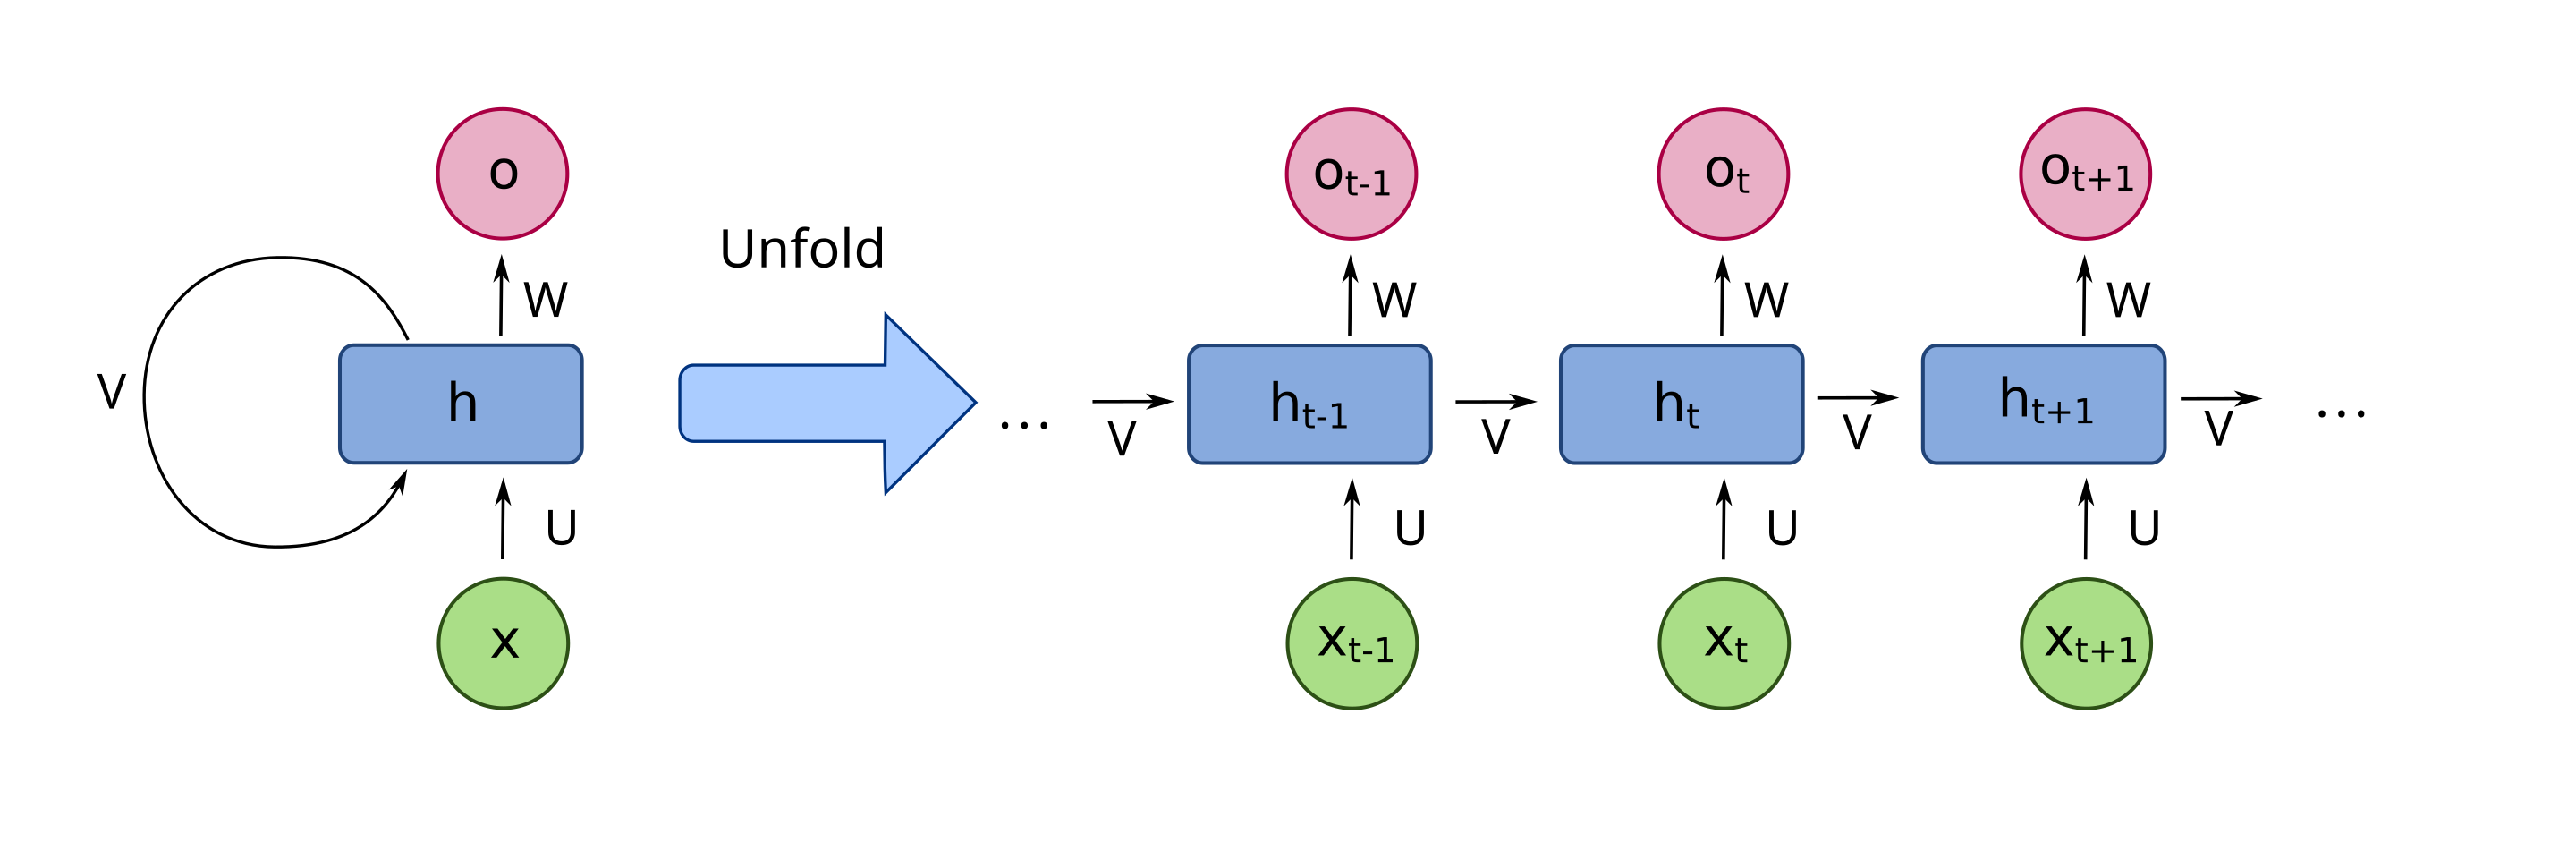
\includegraphics[width=0.8\linewidth]{img/rnn_unfolded.png}
  \caption{A compressed (left) and unfolded (right) RNN}
  \label{fig:rnn_unfolded}
\end{figure}

Abstractly speaking, an RNN is a function $f_{\theta}$ of type $(x_t, h_t) \rightarrow (y_t, h_{t+1})$, where:
\begin{itemize}
  \item $x_t$: input vector.
  \item $h_t$: hidden vector.
  \item $y_t$: output vector.
  \item $\theta$: neural network parameters.
\end{itemize}

It's a neural netowrk that maps an input $x_t$ into an output $y_t$, with the hidden vector $h_t$ playing the role of "memory", a partial record of all previous input-output pairs.
At each step, it transforms input to an output, and modifies its "memory" to help it to better perform future processing.

The figure \ref{fig:rnn_unfolded} may be misleading to many because practical neural netowrk topologies are frequently organized in "layers" and the drawing gives that appearance.
However, what appears to be layers are, in fact, different steps in time, "unfolded" to produce the appearance of layers.

\subsubsection{Bidirectional RNNs}

We can combine two RNNs, one processing the input sequence in one direction, and the other one in the opposite direction
This is called a bidirectional RNN, and it's structured as follows:
\begin{itemize}
  \item The forward RNN processes in one direction: $f_{\theta}(x_0, h_0) = (y_0, h_1), f_{\theta}(x_1, h_1) = (y_1, h_2), ...$
  \item The backward RNN processes in the opposite direction:
  
  ${f'}_{\theta '}(x_N, {h'}_N) = ({y'}_N, {h'}_{N-1}), {f'}_{\theta '}(x_{N-1}, {h'}_{N-1}) = ({y'}_{N-1},{h'}_{N-2}), ...$
\end{itemize}

The two output sequences are then concatenated to give the total output: $((y_0, {y'}_0), (y_1, {y'}_1), ..., (y_N, {y'}_N))$.
A bidirectional RNN allows the model to process a token both in the context of what came before it and what came after it.

\begin{figure}[htbp]
  \centering
  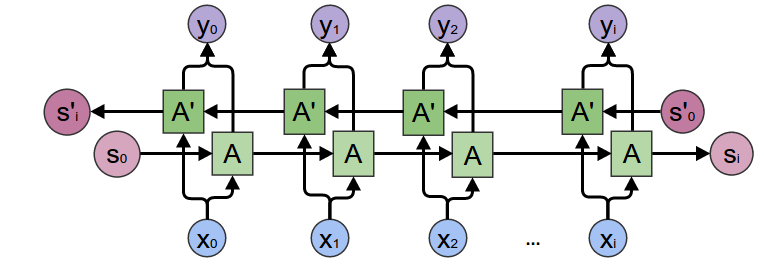
\includegraphics[width=0.8\linewidth]{img/rnn_bidirectional.png}
  \caption{An unfolded bidirectional RNN}
  \label{fig:rnn_bidirectional}
\end{figure}

\subsubsection{LSTM}
\label{sec:lstm}

While Recurrent Neural Networks (RNNs) provide a mechanism for processing sequential data by maintaining a hidden state that captures information from previous steps, they suffer from the vanishing gradient problem.
This issue happens when gradients used to update the network's parameters during training diminish exponentially over time, making it difficult for the network to learn long term dependencies.
To adress this, Long Short-Term Memory (LSTM) networks were introduced as a specialized variant of RNNs.
LSTMs can better capture long-term dependencies by incorporating a more sophisticated memory mechanism and gating structure.

In LSTMs the module, instead of having a single neural network layer, has four parts interacting in a special way.

\begin{figure}[htbp]
  \centering
  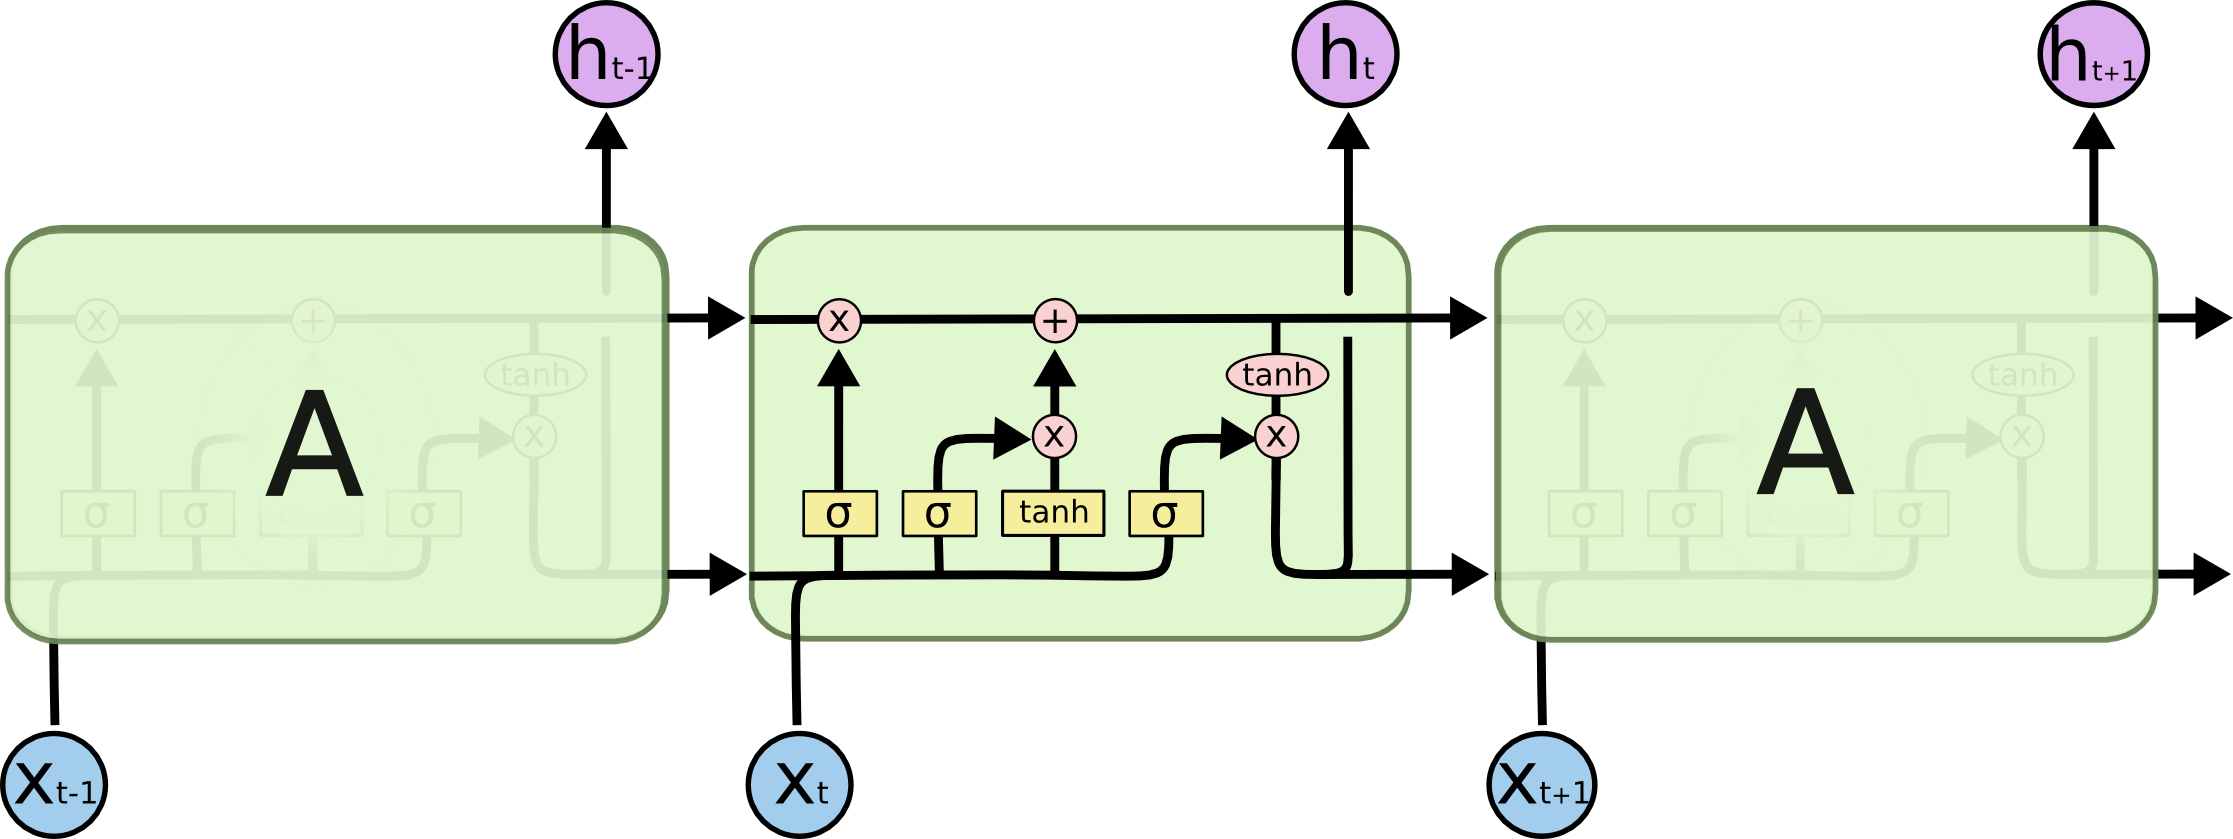
\includegraphics[width=0.8\linewidth]{img/lstm_chain.png}
  \caption{The repeating module in an LSTM}
  \label{fig:lstm_chain}
\end{figure}

In the diagram in figure \ref{fig:lstm_chain}, each line carries an entire vector, from the output of one node to the inputs of others.
The pink circles represent pointwise operations, like vector addition, while the yellow boxes are learned neural network layers.
Lines merging denote concatenation, while a line fork denotes its content being copied and the copies going to different locations.

\paragraph{The core idea behind LSTMs}

The key to LSTMs is the cell state, the horizontal line running through the top of the diagram.
The cell state is like a conveyor belt. It runs straight down the entire chain, with only some minor linear interactions.
It's very easy for information to just flow along it unchanged.

The LSTM does have the ability to remove or add information to the cell state, carefully regulated bu structures called gates.
Gates are a way to optionally let information through.
They are composed out of a sigmoid neural net layer and a pointwise multiplication operation.

The sigmoid layer outputs numbers between zero and one, describing how much of each component should be let through. A value of zero means "let nothing through", while a value of one means "let everything through".
An LSTM has three of these gates, to protect and control the cell state.

\paragraph{The four LSTM parts}
The first step in our LSTM is to decide what information we're going to throw away from the cell state.
This decision is made by a sigmoid layer called the "forget gate layer".
It looks at $h_{t-1}$ and $x_t$ and outputs a number between 0 and 1 for each number in the cell state $C_{t-1}$.
A 1 represents "remember this" while a 0 represents "forget this".

\begin{figure}[htbp]
  \centering
  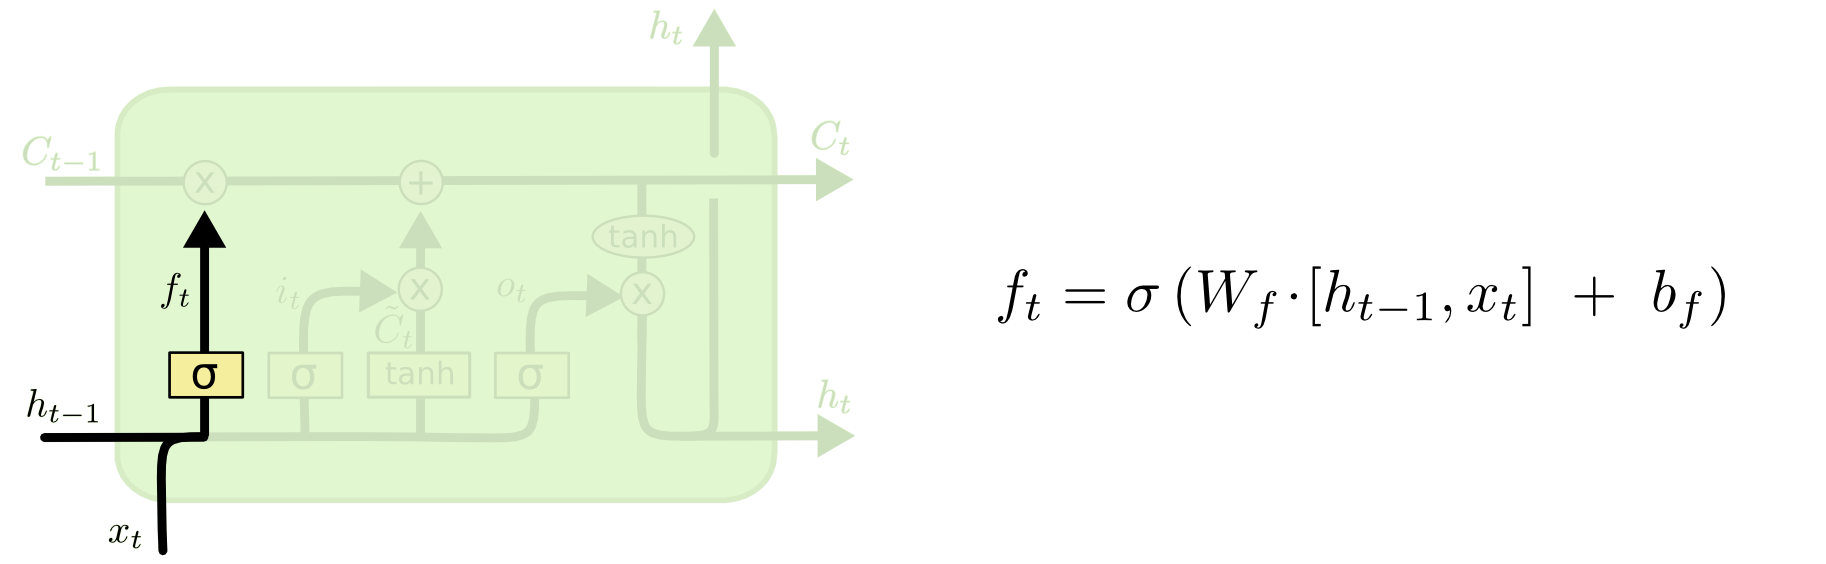
\includegraphics[width=0.6\linewidth]{img/lstm_forget.png}
  \caption{The forget module in an LSTM}
  \label{fig:lstm_forget}
\end{figure}

The next step is to decide what new information we're going to store in the cell state.
This has two parts.
First a sigmoid layer called the "input gate layer" decides which values we'll update.
Next, a tanh layer creates a vector of new candidate values, $\tilde{C}_t$, that could be added to the state.

\begin{figure}[htbp]
  \centering
  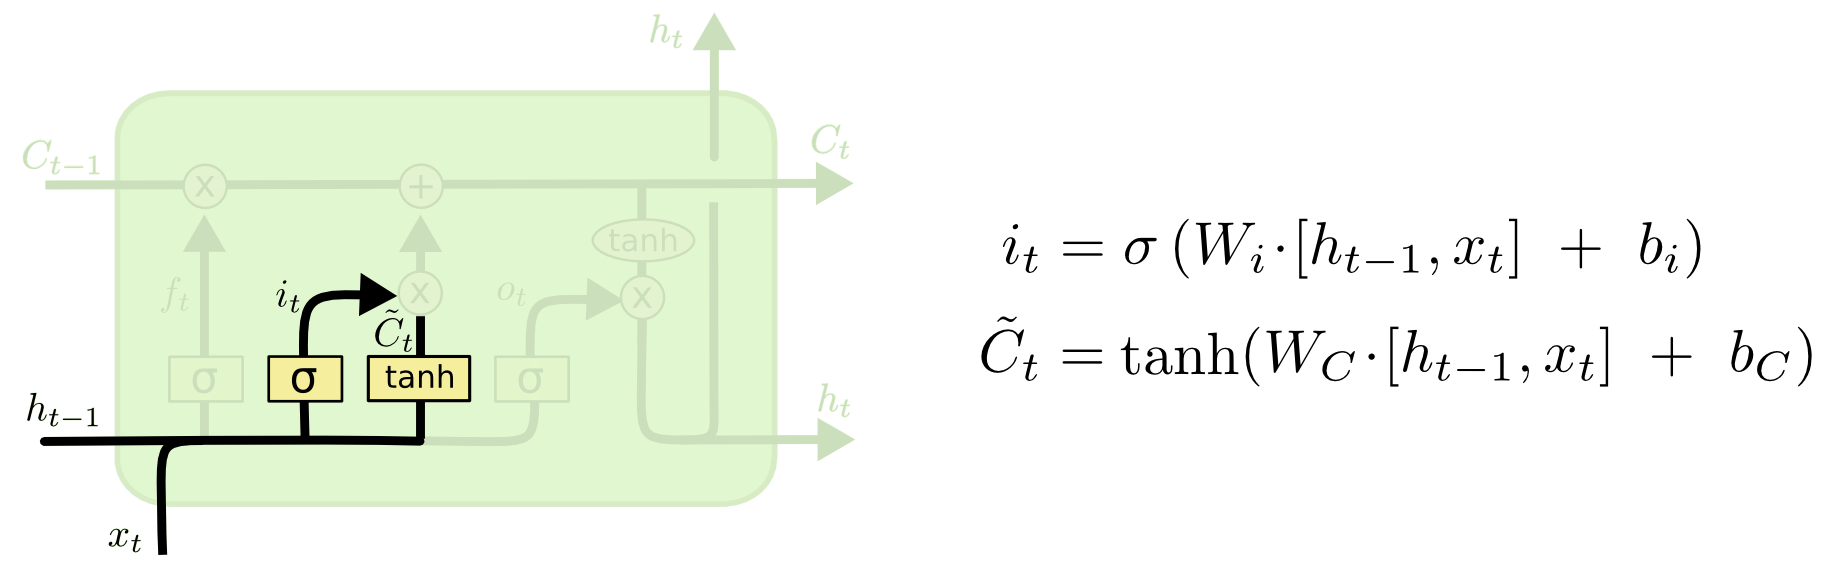
\includegraphics[width=0.6\linewidth]{img/lstm_input.png}
  \caption{The input module in an LSTM}
  \label{fig:lstm_input}
\end{figure}

Next, we have to update the old cell state $C_{t-1}$, into the new cell state $C_t$.
The previous steps already decided what to do, we just need to actually do it.
We multiply the old state by $f_t$, forgetting the things we decided to forget earlier.
Then we add $i_t * \tilde{C}_t$.
This is the new candidate values, scaled by how much we decided to update each state value.

\begin{figure}[htbp]
  \centering
  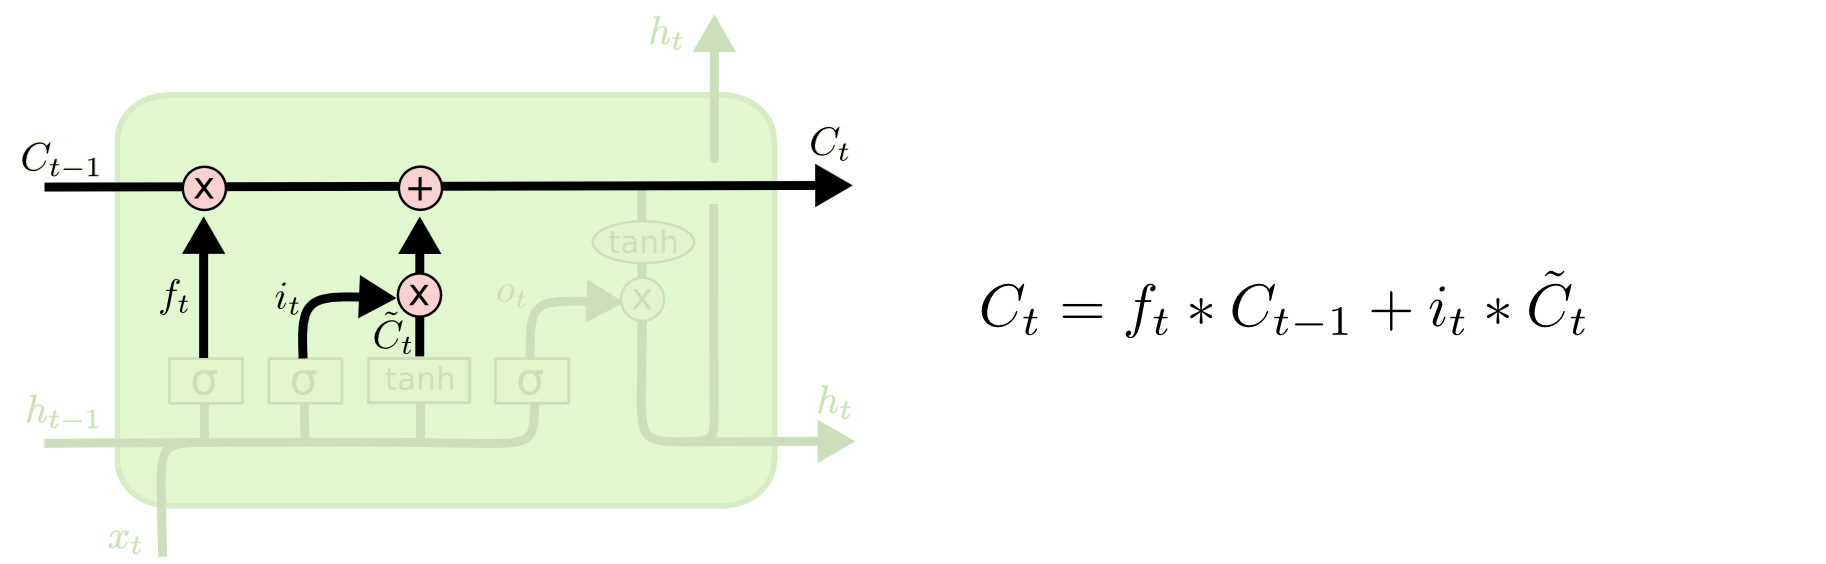
\includegraphics[width=0.6\linewidth]{img/lstm_update.png}
  \caption{The update module in an LSTM}
  \label{fig:lstm_update}
\end{figure}

Finally, we need to decide what we're going to output.
This output will be based on our cell state, but will be a filtered version.
First, we run a sigmoid layer which decides what parts of the cell sate we're going to output.
Then, we put the cell state through tanh (to push the values between -1 and 1) and multiply it by the output of the sigmoid gate, so that we only output the parts we decided to.

\begin{figure}[htbp]
  \centering
  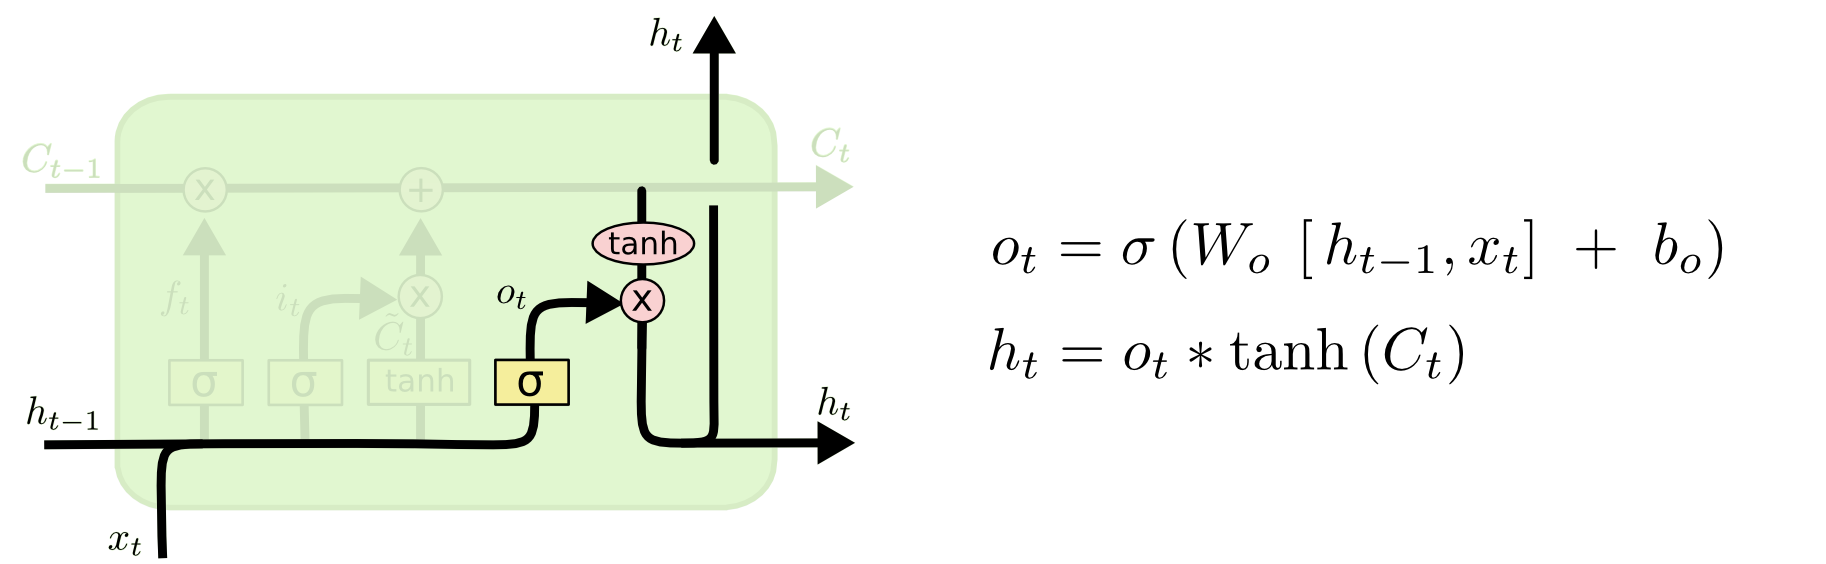
\includegraphics[width=0.6\linewidth]{img/lstm_output.png}
  \caption{The output module in an LSTM}
  \label{fig:lstm_output}
\end{figure}

\section{Technical implementation}

\subsection{Dataset}
IMDB is a popular website that collects movie reviews.
The IMDB dataset is a widely used benchmark for sentiment analysis tasks;
it contains 50000 movie reviews from the website, allowing no more than 30 reviews per movie.
The dataset contains an even number of positive and negative reviews, so randomly guessing yields 50\% accuracy.
Only highly polarized reviews are considered.
A negative review has a score $\leq 4$ out of 10, and a positive review has a score $\geq 7$ out of 10. Neutral reviews are not included in the dataset. \cite{imdb_dataset_stanfordnlp}. 

\subsection{Data preprocessing}

The implementation includes several data preprocessing steps.
Data preprocessing is important because raw textual data often contains noise, suck as typographical errors, inconsistent formatting and irrelevant symbols.
Preprocessing techniques aim to transform raw text data into a clean format that facilitates effective feature extraction and model training.

In this case I cleaned the dataset by removing: links, html tags, double spaces, punctuation and stopwords.
Stopwords are high frequency and low information words such as articles, prepositions, and conjunctions (e.g. "the", "and", "in") that are excluded to reduce noise and improve computational efficiency.
The stopwords were removed by using NLTK (Natural Language ToolKit), a suite of libraries and programs for natural language processing written in Python.
I also lemmatized the dataset.
Lemmatization is the process of reducing words to their root form, known as a lemma.
Unlike stemming, which simply chops off word endings, lemmatization considers the context and part of speech of a word to return a valid dictionary form (e.g. "running" is "run" and "better" is "good").
The entire dataset was also converted to lowercase.

We can see the dataset's head in the following code snippet:
\begin{itemize}
  \item Before the preprocessing:
    \begin{lstlisting}
    0      I rented I AM CURIOUS-YELLOW from my video sto...      0
    1      "I Am Curious: Yellow" is a risible and preten...      0
    2      If only to avoid making this type of film in t...      0
    3      This film was probably inspired by Godard's Ma...      0
    4      Oh, brother...after hearing about this ridicul...      0
    ...                                                  ...    ...
    49995  Just got around to seeing Monster Man yesterda...      1
    49996  I got this as part of a competition prize. I w...      1
    49997  I got Monster Man in a box set of three films ...      1
    49998  Five minutes in, i started to feel how naff th...      1
    49999  I caught this movie on the Sci-Fi channel rece...      1
    \end{lstlisting}

  \item After the preprocessing:
    \begin{lstlisting}
    0      rented curious yellow video store controversy ...      0
    1      curious yellow risible pretentious steaming pi...      0
    2      avoid making type film future film interesting...      0
    3      film probably inspired godard masculin feminin...      0
    4      oh brother hearing ridiculous film umpteen yea...      0
    ...                                                  ...    ...
    49995  got around seeing monster man yesterday long w...      1
    49996  got part competition prize watched really expe...      1
    49997  got monster man box set three film mainly want...      1
    49998  five minute started feel naff looking got comp...      1
    49999  caught movie sci fi channel recently actually ...      1
    \end{lstlisting}
\end{itemize}

\subsection{Model architectures}

\subsubsection{LSTM model}
% Keras provides the necessary components to build a LSTM network.
The proposed model employs a neural network architecture with three core layers, combining embedding, recurrent processing, and final classification.
We will now see the model and go through each one of its layers:
\begin{lstlisting}[language=python]
model = Sequential()
model.add(Embedding(input_dim=TOKENIZER_MAX_WORDS, output_dim=EMBED_DIM))
model.add(LSTM(LSTM_OUT, dropout=0.2, recurrent_dropout=0.2))
model.add(Dense(1, activation="sigmoid"))
model.compile(optimizer="adam", loss="binary_crossentropy", metrics=["accuracy"])
\end{lstlisting}

\paragraph{Embedding layer}
This layer's purpose is to convert integer-encoded word indices into dense vector representations.
The layer learns semantic relationships between words during training.
Instead of having a long, sparse vector, each word is mapped to a dense vector of fixed size.
These vectors are not binary, they contain real numbers that the model learns during training.
Embeddings are powerful because they use vector spaces, so they can capture intricate relationships between words.
For example, in a well trained embedding space, the vector for "king" minus "man" plus "woman" will point to queen.
Embeddings provide a way for the models to understand and relate to the data in a more sophisticated way compared to, for example, one hot encoding \cite{mediumDoesEmbedding}.

\paragraph{LSTM layer}
We have already seen in \ref{sec:lstm} how an LSTM works. 
We know that the LSTM layer processes sequential information while maintaining memory of long-range dependencies.
We add the LSTM layer in the network together with a dropout and recurrent dropout.
Dropout is a regularization technique (a process that converts the answer of a problem to a simpler one) for reducing overfitting in artificial neural networks by preventing complex co-adaptations on training data.
Dropout refers to randomly "dropping out", or omitting, units (both hidden and visible) during the training process of a neural network.
Dropout is the equivalent of training several smaller networks on the same task.
The final model is like an ensemble of smaller networks, reducing variance and providing more robust predictions.
Dropout applies dropout to the non-recurrent connections of the LSTM layer.
Recurrent dropout applies dropout to the recurrent connections (hidden statet transitions) within the LSTM \cite{wikipediaDilutionneural}.

\paragraph{Dense classification layer}
This layer serves as the final classification step.
The dense layer is a fully connected layer that takes the output from the LSTM and maps it to a single scalar value.
The LSTM typically returns a sequence of hidden states or a final hidden state.
This dense layer "summarizes" that information into a single value.
The sigmoid activation function squashes the output into the range $[0,1]$, interpreting it as a probability of the sentiment.

\paragraph{Model compilation}
The model compilation step configures the model for training by defining how it learns (the optimizer), what to optimize for (loss function) and how to evaluate the performance (evaluation metric).
The optimizer is Adam (Adaptive Moment Estimation), an advanced gradient descent alogrithm that adapts learning rates during training.
It combines the benefits of momentum (accelerates updates in consistent gradient directions) and adaptive leraning rates (adjusts rates for each parameter individually).
The loss function is the binary cross-entropy.
The purpose of the loss function is to measure the difference between predicted probabilities and true labels.
It quantifies how well the model performs.
The evaluation metric is the accuracy (the percentage of correct predictions), I didn't choose another metric like F1-score because the dataset is balanced.

\subsubsection{Bidirectional LSTM model}

The bidirectional LSTM model is basically identical to the LSTM network, but it adds a bidirectional layer.
The main difference is that while the standard LSTM processes the sequence in one direction, so it can only capture the past context, while the bidirectional LSTM processes the sequence in both directions, so it can capture both past and future context.
The bidirectional LSTM is more complex, with roughly double the parameters due to the two LSTMs.

\begin{lstlisting}[language=python]
model = Sequential()
model.add(Embedding(input_dim=TOKENIZER_MAX_WORDS, output_dim=EMBED_DIM))
model.add(Bidirectional(LSTM(LSTM_OUT, dropout=0.2, recurrent_dropout=0.2)))
model.add(Dense(1, activation='sigmoid'))
model.compile(optimizer="adam", loss='binary_crossentropy', metrics=['accuracy'])
\end{lstlisting}

\subsection{Hyperparameters selection}
\label{sec:hyperparameters}
% TOKENIZER_MAX_WORDS = 10000
% EPOCHS = 5
% EMBED_DIM = 128
% LSTM_OUT = 64

The network has both fixed and experimented hyperparameters.
The fixed ones are:
\begin{itemize}
  \item \verb|VALIDATION_SPLIT = 0.2|: a small portion (20\% of the training data) is sufficient to evaluate the model's generalization performance without significantly reducing the training set size.
  \item \verb|TOKENIZER_MAX_WORDS = 10000|: Since adults that are native english speakers tend to have a vocabulary of 15000 to 30000 words I expect to be able to extract the positive/negative sentiment with two thirds of the tipical vocabulary \cite{babbelDoesYour}.
\end{itemize}

The hyperparameters where I experimented are:
\begin{itemize}
  \item \verb|BATCH_SIZE|: the batch size is variated from 64 to 128. The batch size defines the number of samples that will be propagated thorugh the network. Using a batch size that is smaller than the number of the samples is useful because it requires less memory since you train the network using fewer samples, and because typically the networks train faster with mini-batches.
  That's because we update the weights after each propagation \cite{stackexchangeWhatBatch}.
  \item \verb|REVIEW_MAX_LENGTH|: the maximum review length is variated from 250 to 500 tokens. A longer sequence allows the model to analyze broader textual patterns. Longer sequences require more memory but reduce the truncation of input text. I chose to test both to determine if longer sequences improve sentiment detection. If 500 improves accuracy, longer sequences are better, if 250 performs similarly, it saves computational resources.
\end{itemize}

This settings challenge the common absumption in deep learning that "bigger is better", that means that a bigger model will yield better results.

\subsection{Model training}
% VALIDATION_SPLIT = 0.2
% K_FOLDS = 5

The model training starts with k-fold cross validation.
Cross validation is a resampling technique used to evaluate machine learning models.
It provides a statistically more reliable estimation of the performance than a single training/test split.
This happens because if we do a single training we could get a particularly easy/hard test set, and so we would not come up with the best estimate possible of the models ability to learn and predict.

We want to use all the data.
So if we use an 80/20 split we are going to do 5-fold cross validation by training the model 5 times on 80\% of the data and testing it on the remaining 20\%.
We ensure that each data point ends up in the 20\% test set exactly once.
We've therefore used every data point we have to contribute to an understanding of how well our model performs the task of learning from some data and predicting some new data \cite{stackexchangeChoosePredictive}.

During model training, since I chose 5 trainng epochs as an arbitrary number, I also used ModelCheckpoint.
This is done or several reasons, in fact using a model checkpoint:
\begin{itemize}
  \item Prevents loss of progress since it saves the model at specified intervals. In fact if training crashes or is interrupted, it can be resumed from the last saved checkpoint instead of starting over.
  \item Saves the "best" model automatically since it only saves the model when the validation loss improves. This is a good thing because it avoids saving suboptimal models, and saves disk space since it overwrites previous checkpoints if the current model has a better validation loss than the last one.
  \item Mitigates overfitting since by monitoring validation loss even if the model starts to overfit after 3 epochs it won't save the final model, that would have degraded performance compared to the one which stopped at 3 epochs.
\end{itemize}

This has been done both for the LSTM and for the bidirectional LSTM.

\section{Results and analysis}

\subsection{Training results}

\subsubsection{LSTM}

As we already pointed out in \ref{sec:hyperparameters}, the LSTM has been trained two times: one with batch size of 64 and maximum review length of 250 and one with batch size of 128 and maximum review length of 500.
These are the training results for the different models and folds:

\begin{table}[H]
  \centering
  \begin{tabular}{c|cccc}
      \toprule
      \textbf{Fold} & \textbf{Accuracy} & \textbf{Precision} & \textbf{Recall} & \textbf{F1-score} \\
      \midrule
      Fold 1 & 0.8710	& 0.8782 & 0.8710 & 0.8704 \\
      Fold 2 & 0.8667	& 0.8698 & 0.8667 & 0.8664 \\
      Fold 3 & 0.8680	& 0.8694 & 0.8680 & 0.8679 \\
      Fold 4 & 0.8603	& 0.8660 & 0.8603 & 0.8598 \\
      Fold 5 & 0.8650	& 0.8652 & 0.8650 & 0.8650 \\
      \midrule
      Mean ($\pm$ std) & 0.866 $\pm$ 0.00396 & 0.870 $\pm$ 0.00515 &	0.866 $\pm$ 0.00396 & 0.866 $\pm$ 0.00395 \\
      \bottomrule
  \end{tabular}
  \vspace{0.5em}
  \caption{LSTM with batch size 64 and review length 250}
\end{table}

\begin{table}[H]
  \centering
  \begin{tabular}{c|cccc}
      \toprule
      \textbf{Fold} & \textbf{Accuracy} & \textbf{Precision} & \textbf{Recall} & \textbf{F1-score} \\
      \midrule
      Fold 1 & 0.8621 & 0.8721 & 0.8621 & 0.8612 \\
      Fold 2 & 0.8484 & 0.8531 & 0.8484 & 0.8479 \\
      Fold 3 & 0.8540 & 0.8641 & 0.8540 & 0.8530 \\
      Fold 4 & 0.8673 & 0.8685 & 0.8673 & 0.8672 \\
      Fold 5 & 0.8701 & 0.8701 & 0.8701 & 0.8701 \\
      \midrule
      Mean ($\pm$ std) & 0.860 $\pm$ 0.00908 & 0.866 $\pm$ 0.00757 & 0.860 $\pm$ 0.00908 & 0.860 $\pm$ 0.00936 \\
      \bottomrule
  \end{tabular}
  \vspace{0.5em}
  \caption{LSTM with batch size 128 and review length 500}
\end{table}

\subsubsection{Bidirectional LSTM}

The bidirectional LSTM has also been trained in the same two configurations as the standard LSTM: one with batch size of 64 and maximum review length of 250 and one with batch size of 128 and maximum review length of 500.
These are the training results for the different models and folds: 

\begin{table}[H]
  \centering
  \begin{tabular}{c|cccc}
      \toprule
      \textbf{Fold} & \textbf{Accuracy} & \textbf{Precision} & \textbf{Recall} & \textbf{F1-score} \\
      \midrule
      Fold 1 & 0.8729 & 0.8760 & 0.8729 & 0.8726 \\
      Fold 2 & 0.8725 & 0.8744 & 0.8725 & 0.8723 \\
      Fold 3 & 0.8637 & 0.8637 & 0.8637 & 0.8637 \\
      Fold 4 & 0.8589 & 0.8590 & 0.8589 & 0.8589 \\
      Fold 5 & 0.8762 & 0.8763 & 0.8762 & 0.8762 \\
      \midrule
      Mean ($\pm$ std) & 0.869 $\pm$ 0.00723 & 0.870 $\pm$ 0.00799 & 0.869 $\pm$ 0.00723 & 0.869 $\pm$ 0.00717 \\
      \bottomrule
  \end{tabular}
  \vspace{0.5em}
  \caption{Bidirectional LSTM with batch size 64 and review length 250}
\end{table}

\begin{table}[H]
  \centering
  \begin{tabular}{c|cccc}
      \toprule
      \textbf{Fold} & \textbf{Accuracy} & \textbf{Precision} & \textbf{Recall} & \textbf{F1-score} \\
      \midrule
      Fold 1 & 0.8746 & 0.8780 & 0.8746 & 0.8743 \\
      Fold 2 & 0.8465 & 0.8482 & 0.8465 & 0.8463 \\
      Fold 3 & 0.8675 & 0.8700 & 0.8675 & 0.8673 \\
      Fold 4 & 0.8508 & 0.8629 & 0.8508 & 0.8495 \\
      Fold 5 & 0.8728 & 0.8728 & 0.8728 & 0.8728 \\
      \midrule
      Mean ($\pm$ std) & 0.862 $\pm$ 0.01295 & 0.866 $\pm$ 0.01153 & 0.862 $\pm$ 0.01295 & 0.862 $\pm$ 0.01322 \\
      \bottomrule
  \end{tabular}
  \vspace{0.5em}
  \caption{Bidirectional LSTM with batch size 128 and review length 500}
\end{table}

\subsection{Training curves}

We can look at the training curves to make an initial qualitative analysis.
The data has been obtained by computing the average of the accuracy/loss and validation accuracy/validation loss, if they were present in the data that has been collected.

\subsubsection{LSTM}

\begin{figure}[H]
  \centering
  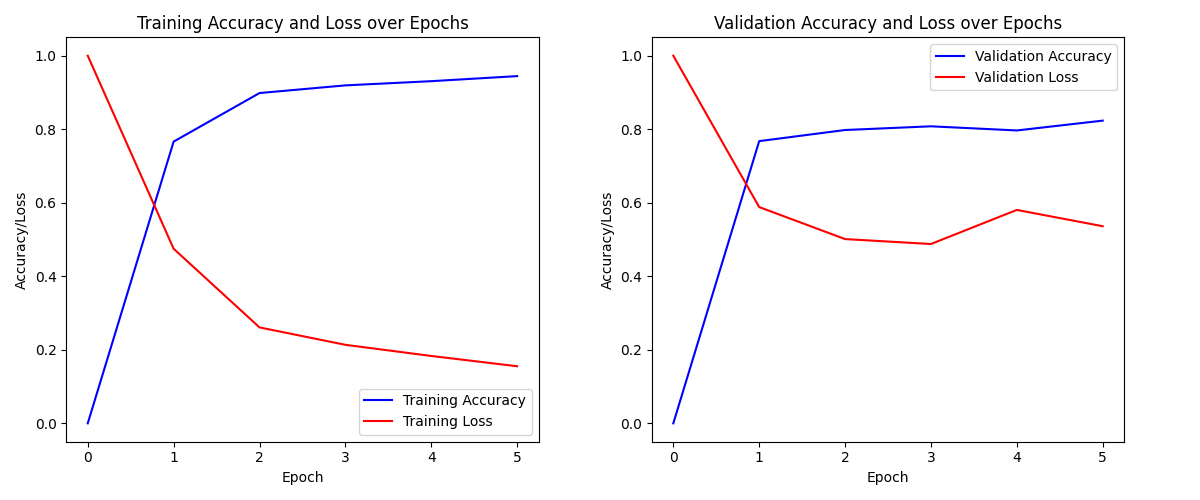
\includegraphics[width=0.9\linewidth]{img/training_curves_lstm_64_250.png}
  \caption{Training and validation set accuracy and loss for LSTM with batch size 64 and review length 250}
  \label{fig:training_curves_lstm_64_250}
\end{figure}

\begin{figure}[H]
  \centering
  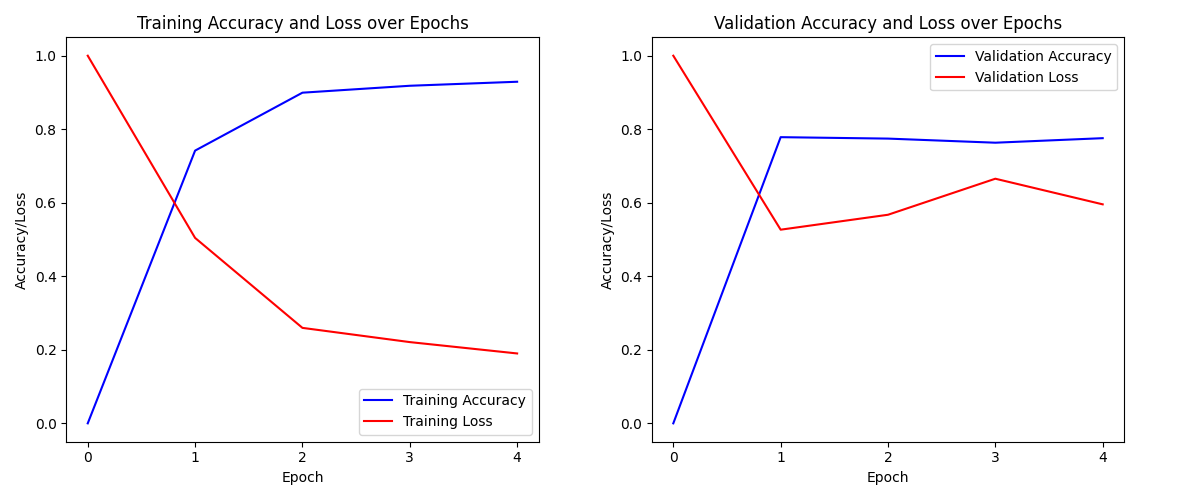
\includegraphics[width=0.9\linewidth]{img/training_curves_lstm_128_500.png}
  \caption{Training and validation set accuracy and loss for LSTM with batch size 128 and review length 500}
  \label{fig:training_curves_lstm_128_500}
\end{figure}

By looking at \ref{fig:training_curves_lstm_64_250} and \ref{fig:training_curves_lstm_128_500} we can make some considerations:

\paragraph{Training set performance}
In both figure \ref{fig:training_curves_lstm_64_250} and figure \ref{fig:training_curves_lstm_128_500} the model shows rapid initial learning in the first two epochs, with training accuracy increasing sharply to approximately 90\% accuracy.
The training loss correspondingly descreases steeply during this period.
After the first two epochs, the improvement becomes more gradual, with training accuracy continuing to climb slowly and eventually reaching around 95\% by epoch 5.
The training loss continues to decrease steadily, reaching the value of about 15\%.

\paragraph{Validation set performance}
The validation metrics show a different pattern.
While there is also a sharp improvement in the first two epochs (most of which comes from the first one), the validation accuracy plateaus at around 0.8 and shows minimal improvement after that.
The validation loss is more concerning.
In fact, after its initial decrease, stabilizes at much higher value compared to the training loss for both \ref{fig:training_curves_lstm_64_250} and \ref{fig:training_curves_lstm_128_500}.
Also, we can see that in figure \ref{fig:training_curves_lstm_64_250} the curve for the validation accuracy is smoother than the one in \ref{fig:training_curves_lstm_128_500}.
The same can be said for validation loss, that increases after the first epoch in \ref{fig:training_curves_lstm_128_500}, and in \ref{fig:training_curves_lstm_64_250} continues to go down for three epochs.

\paragraph{Signs of overfitting}
There are clear indicators of overfitting in these curves.
The growing gap between training and validation accuracy, combined with the significant difference between training and validaiton loss, suggests the model is memorizing the training data rather than learning generalizable patterns.

\paragraph{Mitigating the overfitting}
Based on these patterns the early stopping I implemented in the models was a really good choice, since it stopped the training most of the time after 3 epochs.
In fact, of the 10 different trainings, only one reached 5 epochs, three reached 4 epochs and the remaining six stopped at 3 epochs.

\subsubsection{Bidirectional LSTM}

\begin{figure}[H]
  \centering
  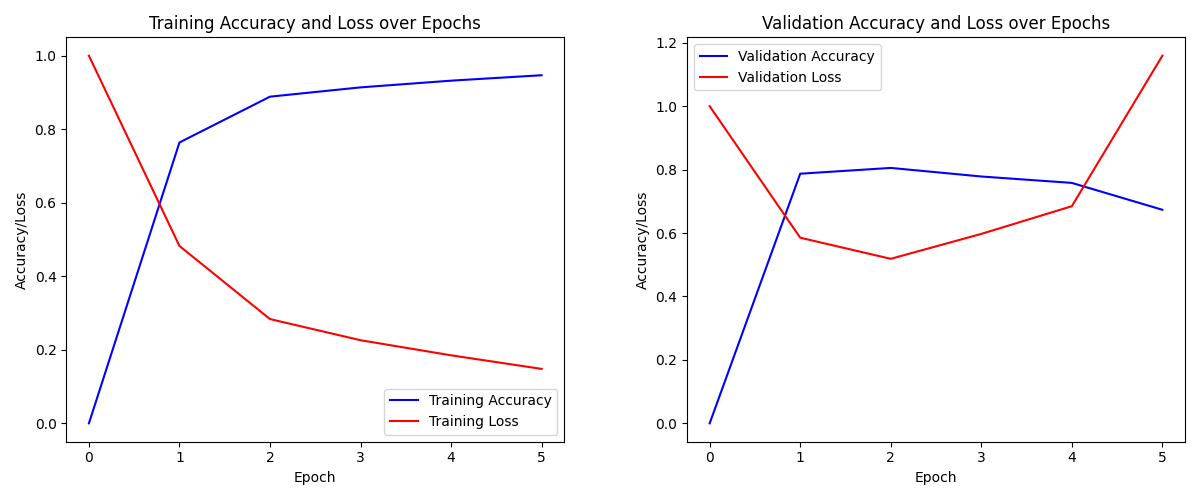
\includegraphics[width=0.9\linewidth]{img/training_curves_bidirectional_64_250.png}
  \caption{Training and validation set accuracy and loss for bidirectional LSTM with batch size 64 and review length 250}
  \label{fig:training_curves_bidirectional_64_250}
\end{figure}

\begin{figure}[H]
  \centering
  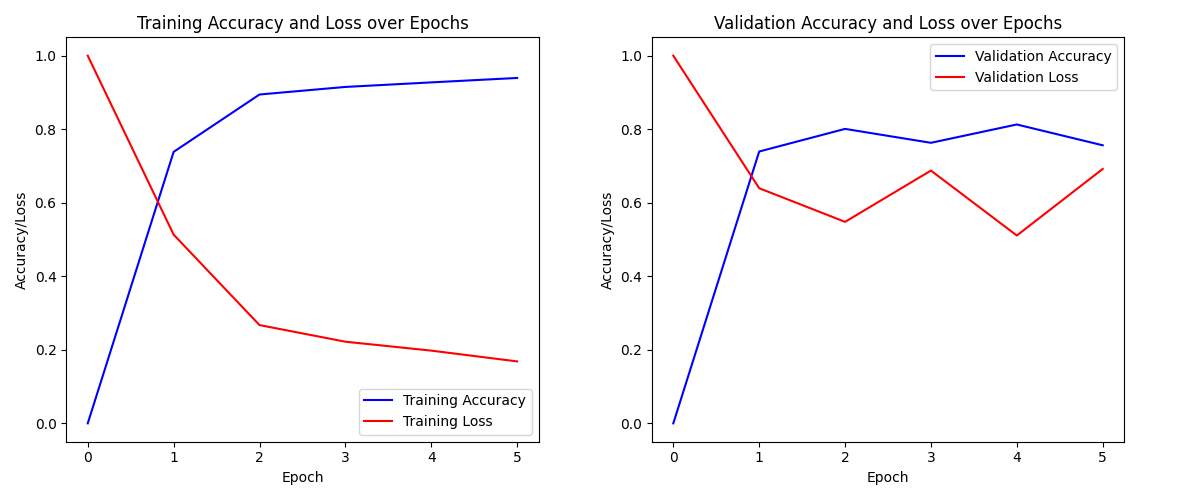
\includegraphics[width=0.9\linewidth]{img/training_curves_bidirectional_128_500.png}
  \caption{Training and validation set accuracy and loss for bidirectional LSTM with batch size 128 and review length 500}
  \label{fig:training_curves_bidirectional_128_500}
\end{figure}

For \ref{fig:training_curves_bidirectional_64_250} and \ref{fig:training_curves_bidirectional_128_500} we can make considerations similar to what we did for the LSTM curves, since we can see a similar behaviour of rapidly approaching convergence, and then overfitting.
This is even more visible in the bidirectional LSTM, that starts to lose accuracy and gain loss in the validation sets after convergence, a thing that didn't happen that much in the LSTM.

\subsection{Results analysis}

Just by looking at the previous results I think that I got a decent model, but I also think that I could try to get a better one if I tuned the network hyperparameters to train the models more slowly, so that the model doesn't risk overshooting the optimal result.

Let's proceed with a more technical analysis.
We will do a Wilcoxon signed-rank test, first to compare if the bigger model is better as we expected to be, and then if the model we found was better in normal or bidirectional configuration.
Also we discovered that in our case the review length at 250 is enough to extrapolate the sentiment, and doubling the sequence length doesn't give an improvement.

The Wilcoxon test on the LSTM with batch size 64 and maximum text size 250 and the LSTM with batch size 128 and maximum test size 500 returns a p-value of 0.316.
We can also see the boxplots to see how the performance varies across folds.

\begin{figure}[htbp]
  \centering
  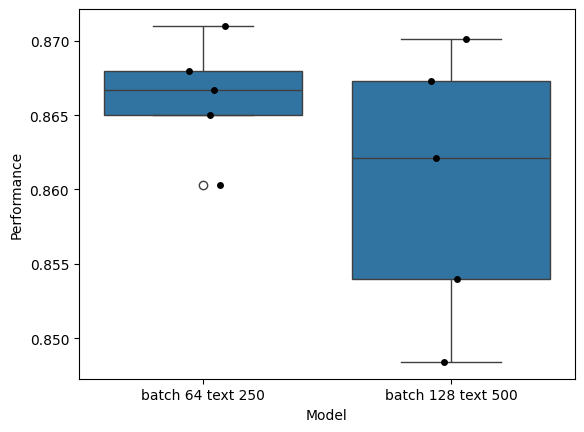
\includegraphics[width=0.6\linewidth]{img/boxplot_lstm.png}
  \caption{The boxplot of the LSTM}
  \label{fig:lstm_boxplot}
\end{figure}

Since the two models perform similarly, we choose the one with fewer parameters for two reasons: it has a lower variance (so we expect that it will yield more consistent results) and it's simpler so we follow the Occam's razor principle.

By performing the same analysis on the bidirectional LSTM we get a p-value of 0.438 and so we fail again to reject the null hypothesis. We can choose the simpler bidirectional LSTM again for the reasons stated above.
We can see the boxplots of the bidirectional LSTMs.

\begin{figure}[htbp]
  \centering
  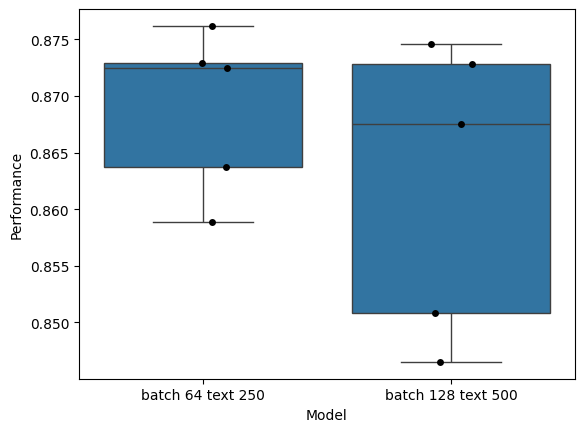
\includegraphics[width=0.6\linewidth]{img/boxplot_bidirectional.png}
  \caption{The boxplot of the bidirectional LSTM}
  \label{fig:bidirectional_boxplot}
\end{figure}

Now we can compare the LSTM with batch size 64 and text length of 250 with its bidirectional LSTM counterpart.
Doing so results in a p-value of 0.438, so again we reject the null hypothesis.
We can again choose the simpler model (the LSTM) and plot the boxplots.

\begin{figure}[htbp]
  \centering
  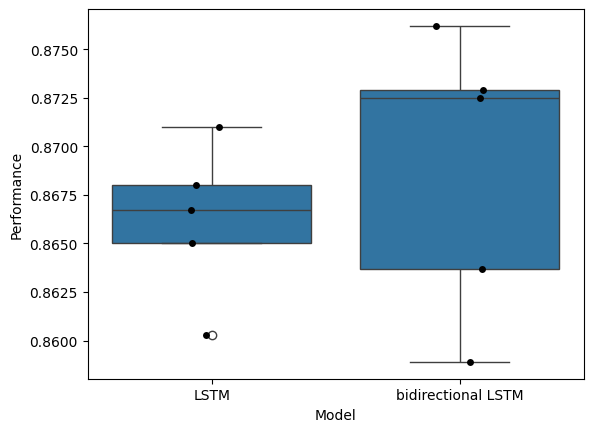
\includegraphics[width=0.6\linewidth]{img/boxplot_comparison.png}
  \caption{The boxplot of the LSTM and the bidirectional LSTM}
  \label{fig:comparison_boxplot}
\end{figure}

\section{Conclusions}

I started by thinking that a bigger model would have given me a better model, and I found out that this was not the case this time.
Some doubts still remain because we have seen that the models converge really fast, but further hyperparameters tuning and analysis would be necessary to say this without any doubts.

If we compare the results with the results of the paper that introduced the IMDB dataset, we can see that they achive 87.44\% accuracy on the dataset with a model that combines unsupervised and supervised techniques to learn word vectors that capture both semantic and sentiment information \cite{imdb_dataset_stanfordnlp}.

I found also an implementation on Kaggle that uses logistic regression with Tfidf for text vectorization and gets 90\% accuracy on the test set. Unfortunately I couldn't verify my LSTM against theirs since they fitted the tokenizer on the whole dataset, and not just the training set, so i think their performance could be improved by that \cite{kaggleIMDbSentiment}.

I found another interesting implementation that uses again logistic regression with 89.03\% accuracy, and also tried to use a LSTM.
Even if their training curves look nicer than mine and they use also batch normalization, conv and max pooling, their accuracy on the test set is 87.78\%, so not much different from my result.
Finally, they also use BERT, which yields 89.85\% accuracy on the test set \cite{kaggleIMDBSentimentLSTMandBERT}.

\bibliographystyle{unsrt}
\bibliography{references.bib}

\end{document}
